\documentclass[options]{report}

\usepackage[a4paper, total={6in, 8in}]{geometry}
\usepackage{amsmath}
\usepackage{graphicx}

\title{{\large Master Thesis} \\ 3D human interaction synthesis \\ for action recognition data augmentation}


\newcommand{\norm}[2]{\left \lVert #1 \right \rVert_{#2}}

\DeclareMathOperator*{\argmax}{argmax\,}
\DeclareMathOperator*{\argmin}{argmin\,}

\author{Anders Bredgaard Thuesen}
\date{\today}


\begin{document}
\maketitle

\section*{Abstract}

\section*{Introduction}


\section*{Data}


\section*{Methods}

\subsection*{SMPL \& Human Mesh Reconstruction }
\begin{figure}[h]
    \centering
    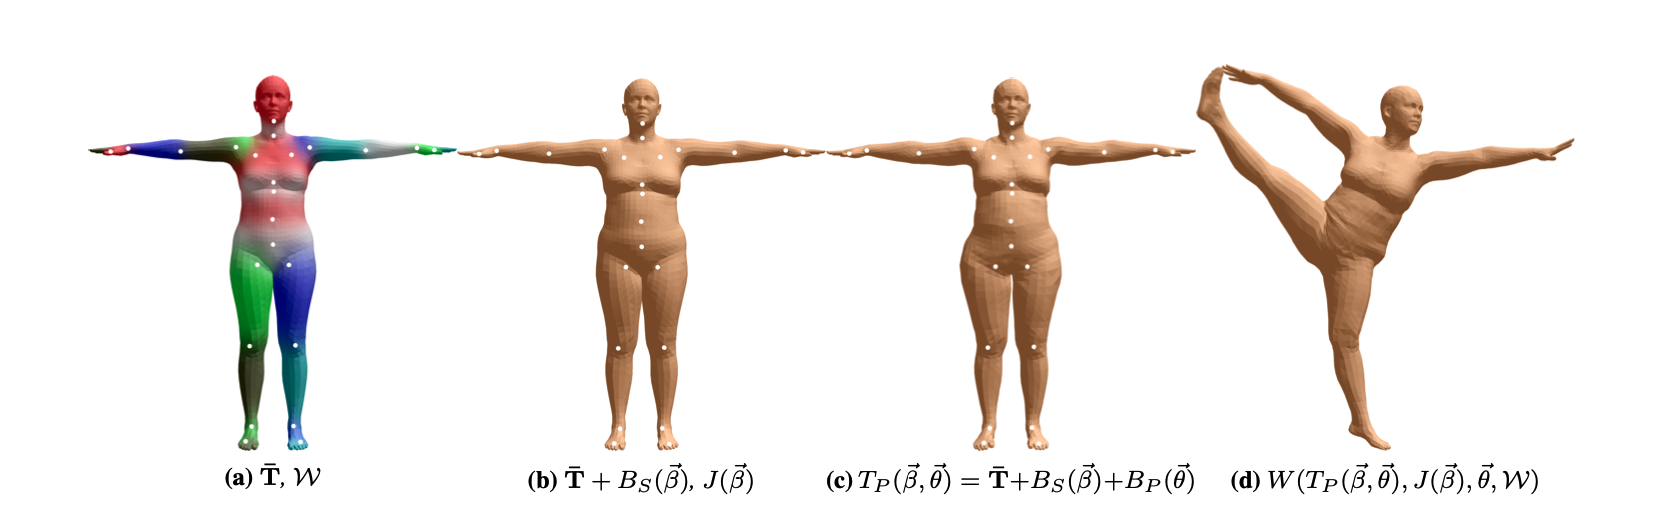
\includegraphics[width=\linewidth]{figures/smpl.png}
    \caption{SMPL model}
\end{figure}
The Skinned Multi-Person Linear (SMPL) model is a parametric body shape model that accurately represents a wide range of human bodies and poses. It is built upon a foundation of linear blend skinning enhanced with corrective blend shapes, which are derived from a large dataset of body scans. The model captures the subtle deformations that occur with different body shapes and poses and can easily be rendered due to its compatibility with existing graphics pipelines. Since its publication, several extensions such as DMPL, incorporating dynamic soft-tissue deformation and SMPL-X, also modelling hands and facial expressions have been introduced. The model is parameterized by $\vec{\beta}$, capturing the variations from a mean body shape and $\vec{\theta}$, specifying the axis-angle rotation of 23 of the template skeleton joints. Mathematically, the model can be expressed as:
\begin{equation}
    M(\vec{\beta}, \vec{\theta}) = W(T_P(\vec{\beta}, \vec{\theta}), J(\vec{\beta}), \vec{\theta}, \mathcal{W})
\end{equation}
where $T_P(\vec{\beta}, \vec{\theta})$ returns the vertices of the rest pose, incorporating the deformations from the body shape and pose and is given by:
\begin{equation}
    T_P(\vec{\beta}, \vec{\theta}) = \mathbf{\bar{T}} + B_S(\vec{\beta}) + B_P(\vec{\theta})
\end{equation}
$J(\vec{\beta})$ returns the 3D joint locations from the shaped template vertices using a learned regression matrix $\mathcal{J}$ and is given by:
\begin{equation}
    J(\vec{\beta}) = \mathcal{J}(\mathbf{\bar{T}} + B_S(\vec{\beta}))
\end{equation}
$W$ is the skinning function (e.g. Linear Blend Skinning (LBS) or Dual-Quaternion Blend Skinning (DQBS)) and $\mathcal{W}$ is the blend weights. 


\subsection*{Tracking \& Matching}
We track the predicted staff and patients across multiple frames, indicated by $t = 1 \ldots T$, by iteratively assigning the predictions, $\{ P_i^{(t)} \}_{i=1}^{M_t}$, to the latest known tracks, $\{ Q^{(t)}_{j} \}_{j=1}^{N_t}$ by greedily picking the assignment with the minimum cost:
\begin{equation}
    \argmin_{i,j} \mathcal{L}_\text{track}(P^{(t)}_i, Q^{(t-1)}_j),
\end{equation}
until either all predictions or latest tracks have been assigned exactly once. In the case of any unassigned predictions, a new track is initialized. After tracks have been assigned, the latest track $Q^{(t)}_j$ is updated with the assigned predictions. We choose the following composite loss function:
\begin{equation}
    \mathcal{L}_\text{track}(P, Q) = \alpha \norm{P_\text{3D kpts} - Q_\text{3D kpts}}{2} + \beta \norm{P_\text{class} - Q_\text{class}}{\infty},
\end{equation}
incorporating both the Euclidean distance between the 3D joint keypoints as well as the predicted person class (staff/patient), with $\alpha$ and $\beta$ weighting the influence of each term. The tracks, $T_i$, are then greedily matched to the ground truth annotations $G_j$, minimizing the loss:
\begin{equation}
    \mathcal{L}_\text{match}(T, G) = \sum_t^{T} \begin{cases}
        \norm{a^{(t)}_{\text{track}, \text{2D kpts}} - b^{(t)}_{\text{track}, \text{2D kpts}}}{2} & \text{if}\ a^{(t)}_\text{track} \in a_\text{track} \\
        \gamma & \text{otherwise}
    \end{cases}
\end{equation}
over the trajectory time horizon $t = 1,2,\ldots,T$ where $\gamma$ is the punishment for not detecting the person.



\subsection*{Denoising Diffusion Probabilistic Models (DDPM)}
\begin{enumerate}
    \item Forward and backwards process 
    \item Noise schedule
    \item ELBO derivation
\end{enumerate}

\subsection*{Tranformer}
\subsection*{Rotary Positional Encodings (RoPE)}
\subsection*{Network architecture}




\end{document}